\subsection{Real-time Execution of \ourmethod}
\label{subsec:realtime}

Diffusion-based WAMs inherit powerful generalization from video foundation models, but their iterative denoising process creates a fundamental tension with reactive robotic control. We address two questions: (1) What prevents WAMs from being reactive policies? (2) How do we resolve this for real-time control?

\subsubsection{The Reactivity Gap}

Reactive policies must respond to environmental changes within tens of milliseconds. A naive implementation of \ourmethod on a single GPU requires approximately 5.7 seconds per action chunk due to three bottlenecks: (1) iterative denoising across 16 diffusion steps required for smooth actions, (2) the computational cost of a 14B parameter DiT backbone, and (3) sequential execution that blocks robot motion during inference. This latency makes closed-loop control infeasible.\footnote{One might expect that generating only actions (not video) would accelerate inference, but at 14B scale we empirically found out that the speed gain is minimal—the number of diffusion steps and the number of DiT blocks dominate latency. Moreover, because video and action are jointly trained for strong cross-modal alignment, naively reducing action denoising steps degrades quality. This motivates \ourmethod-Flash.}

\subsubsection{Asynchronous Closed-Loop Execution}

Our first step towards resolving this is through asynchronous execution that decouples inference from action execution. Rather than waiting for each inference to complete, the motion controller continuously executes the most recent action chunk while inference runs concurrently on the latest observation. This structure transforms the latency constraint from ``inference must complete before the robot moves'' to ``inference must complete before the current action chunk expires.'' In our experiments, we deploy policies at an action horizon of 48 steps at 30Hz control frequency (1.6 seconds per chunk) for bimanual manipulation robots. Hence, we target inference latency below approximately 200ms to ensure sufficient overlap for smooth, reactive control.

\subsubsection{System-level Optimizations}

Given the asynchronous execution structure, we optimize inference throughput through parallelism and caching.

\begin{itemize}
    \item \textbf{CFG Parallelism.} Classifier-free guidance \citep{ho2022classifier} requires two forward passes (conditional and unconditional). We distribute these across two GPUs, reducing per-step latency by 47\%.
    \item \textbf{DiT Caching.} We exploit the directional consistency of velocity predictions during flow matching. When cosine similarity between successive velocities exceeds a threshold, we reuse cached velocities, reducing effective DiT steps from 16 to 4 with minimal quality loss on action prediction.
\end{itemize}

\subsubsection{Implementation-level Optimizations}

We further reduce latency through compiler and kernel enhancements.
\begin{itemize}
    \item \textbf{Torch Compile and CUDA Graphs.} We apply \texttt{torch.compile} with CUDA Graphs to eliminate CPU overhead and fuse operators. Static shapes cause recompilations only during the first trajectory.
    \item \textbf{Post-Training Quantization.} On Blackwell architecture, we quantize weights and activations to NVFP4 while keeping sensitive operations (QKV, Softmax) in FP8 and non-linear operations in FP16.
    \item \textbf{Kernel and Scheduler Enhancements.} We use the cuDNN backend for attention and migrate scheduler operations to GPU to eliminate CPU-GPU synchronization stalls.
\end{itemize}
\begin{figure}[h!]
    \centering
    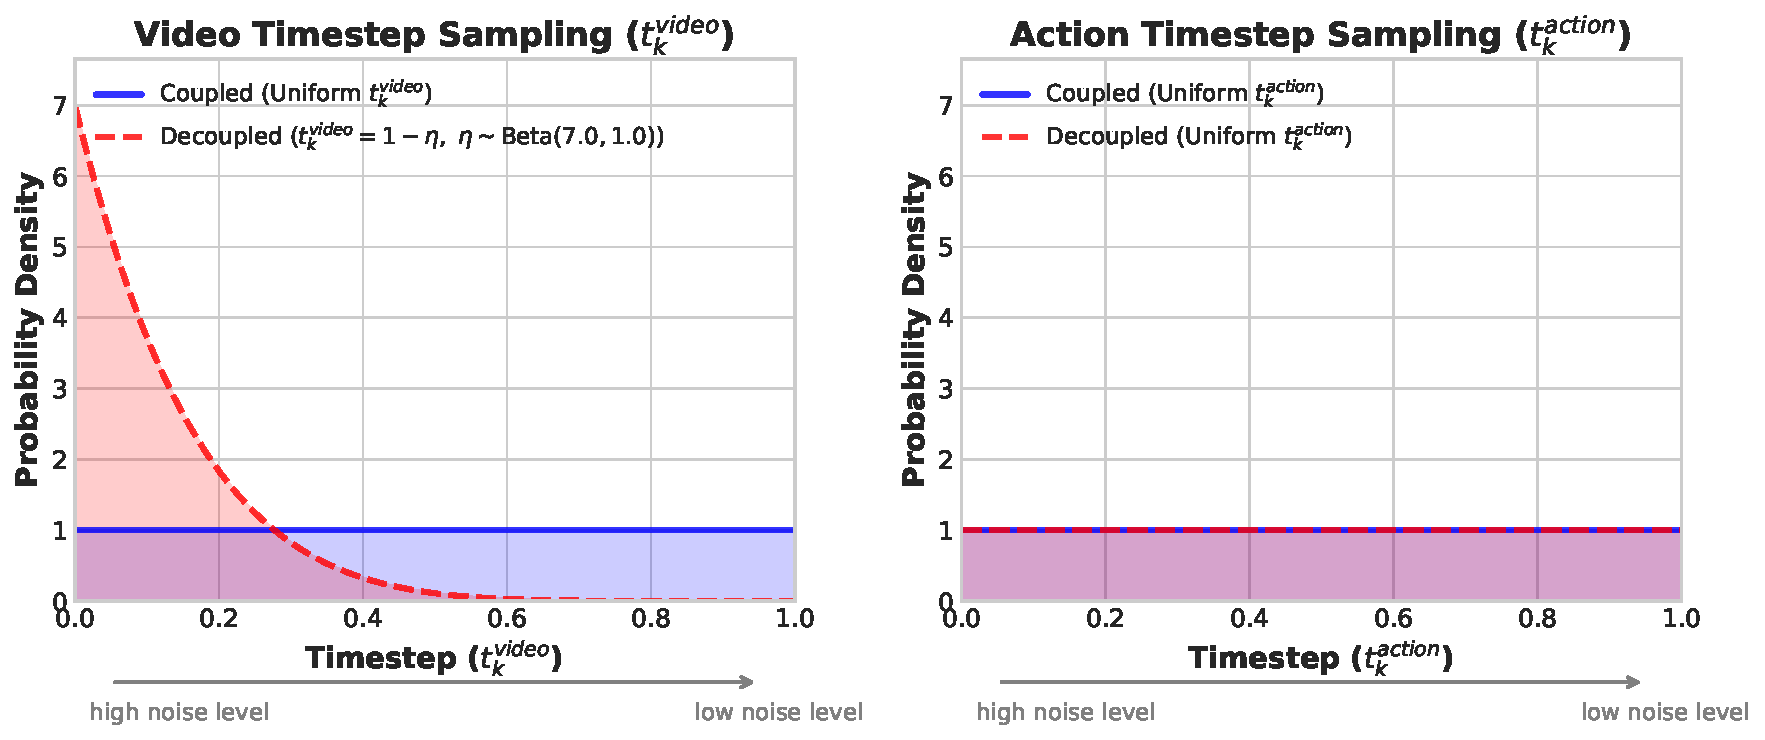
\includegraphics[width=0.8\textwidth]{figures/dreamzero-flash_noise_distribution-comparison.pdf}
    \caption{\textbf{Decoupled Noise Schedules.} \ourmethod (blue) uses coupled noise for video and action (both uniform). \ourmethod-Flash (red) biases video toward high-noise states via a Beta distribution while keeping action noise uniform, training the model to predict clean actions from noisy visual context.}
    \label{fig:dreamzeroflash}
\end{figure}
\subsubsection{Model-level Optimizations: \ourmethod-Flash}
\label{subsec:dreamzeroflash}



Even with system optimizations, the number of diffusion steps remains the primary latency bottleneck. However, naively reducing steps degrades action quality because residual visual noise propagates into action predictions.

\ourmethod-Flash addresses this by decoupling video and action noise schedules during training. 
The key insight is that, at inference time, actions should denoise to their final values while being conditioned on a still-noisy video representation within the current chunk, since with very few denoising steps (e.g., fewer than 4), the generated video tokens may remain inaccurate and thus provide a noisy conditioning signal.
Standard \ourmethod samples a shared timestep $t_k \sim \mathcal{U}(0,1)$ for both modalities. This creates a train-test mismatch: during training, the model learns to predict actions when video and action are at the \textit{same} noise level, but few-step or single-step inference requires predicting clean actions while video remains partially noisy.

\ourmethod-Flash closes this gap by biasing video timesteps toward high-noise states via $t_k^{\text{video}} = 1 - \eta$, where $\eta \sim \text{Beta}(\alpha, \beta)$ with $\alpha > \beta$.
In practice, we use $\text{Beta}(7, 1)$ as an example configuration, yielding $\mathbb{E}[t_k^{\text{video}}] = 0.125$ (predominantly noisy), while action timesteps remain uniform (Figure~\ref{fig:dreamzeroflash}). During training, this exposes the model to configurations where it must predict clean actions from noisy visual context, directly matching the few-step or single-step inference regime. As a result, we reduce the diffusion steps from four to one, cutting inference from ${\sim}350$ms to ${\sim}150$ms with minimal performance loss (Table~\ref{tab:tidying_one_step}). Moreover, the Flash formulation enables flexible training configurations—such as varying the noise sampling ratios of video and action—to better align training with different few-step or single-step inference regimes. In practice, we mainly apply Flash training as the final stage following the main \ourmethod model training.

\textbf{Action Chunk Smoothing.} To suppress high-frequency noise in generated actions, we upsample chunks to $2\times$ resolution, apply a Savitzky-Golay filter, and downsample to original resolution.

\subsubsection{Summary}

Table~\ref{tab:inference_speedup} summarizes cumulative speedups. System and implementation optimizations yield ${\sim}9\times$ speedup on H100 and ${\sim}16\times$ on GB200; adding \ourmethod-Flash achieves 38$\times$ on GB200, reducing latency from 5.7s to 150ms. With the exception of DiT caching and quantization, all system and implementation-level optimizations are mathematically equivalent to baseline and show no measurable performance degradation.

\begin{table}[h]
\centering
\begin{threeparttable}
\begin{tabular}{@{}lcc@{}}
\toprule
\textbf{Optimization} & \textbf{H100} & \textbf{GB200}\\ 
\midrule
Baseline & 1$\times$ & 1.1$\times$ \\
\midrule
\multicolumn{3}{l}{\textit{System-level}} \\
\quad + CFG Parallelism  & 1.9$\times$ & 1.8$\times$ \\
\quad + DiT Caching & 5.5$\times$  & 5.4$\times$ \\
\midrule
\multicolumn{3}{l}{\textit{Implementation-level}} \\
\quad + Torch Compile + CUDA Graphs & 8.9$\times$ & 10.9$\times$ \\
\quad + Kernel \& Scheduler Opts. & 9.6$\times$ & 14.8$\times$ \\
\quad + Quantization (NVFP4) & — & 16.6$\times$ \\ 
\midrule
\multicolumn{3}{l}{\textit{Model-level}} \\
\quad + \ourmethod-Flash & — & 38$\times$ \\
\bottomrule
\end{tabular}
\caption{\textbf{Cumulative inference speedups.} Each row includes all optimizations above it. Entries marked ``—'' indicate features not applicable to that hardware.}
\label{tab:inference_speedup}
\end{threeparttable}
\vspace{-0.1in}
\end{table}